% State diagram of the bnn_top controller (P = 1).
% Build (from docs/):  pdflatex -output-directory=../build/latex state_diagram_p1.tex
% Plain article class (no standalone.cls needed); the PDF page is sized to the
% diagram at the end of the file.
\documentclass{article}
\usepackage{tikz}
\usetikzlibrary{arrows.meta,calc}
\pagestyle{empty}
\newsavebox{\diagram}

\tikzset{
  >={Stealth[length=2.4mm]},
  every node/.style={font=\small},
  state/.style={circle,draw,very thick,fill=red!6,minimum size=17mm,font=\bfseries},
  outs/.style ={draw,thick,fill=blue!6,rounded corners=2pt,font=\scriptsize,align=center,inner sep=3pt},
  tr/.style   ={->,thick},
  cond/.style ={font=\small},                                  % transition condition
  act/.style  ={font=\scriptsize,text=red!65!black,align=center}, % register updates on that edge
}
% NOT, written as an overbar
\newcommand{\nt}[1]{\ensuremath{\overline{\mathit{#1}}}}
\newcommand{\sg}[1]{\ensuremath{\mathit{#1}}}

\begin{document}
\begin{lrbox}{\diagram}
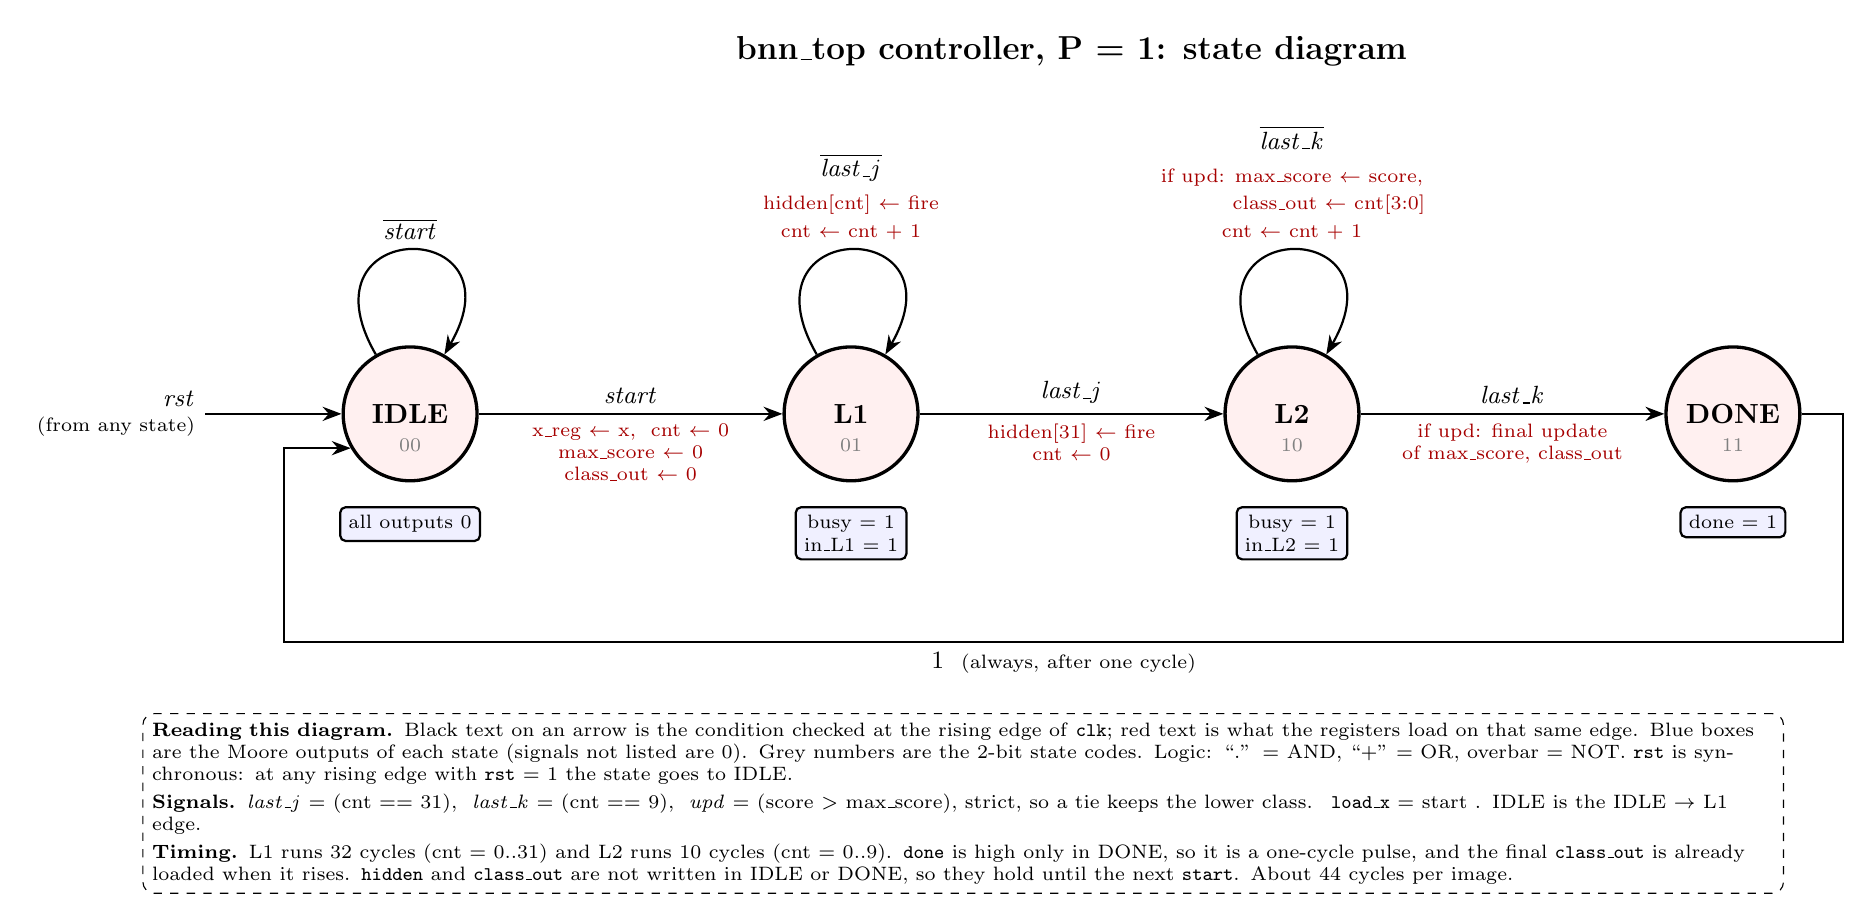
\begin{tikzpicture}

\node[font=\large\bfseries] at (8.4,4.6) {bnn\_top controller, P = 1: state diagram};

% ---------------------------------------------------------------- states
\node[state] (idle) at (0,0)    {IDLE};
\node[state] (l1)   at (5.6,0)  {L1};
\node[state] (l2)   at (11.2,0) {L2};
\node[state] (done) at (16.8,0) {DONE};

% state codes
\foreach \s/\c in {idle/00, l1/01, l2/10, done/11}
  \node[font=\scriptsize,text=gray] at ([yshift=-4mm]\s.center) {\c};

% Moore outputs (only the signals that are 1; everything else is 0)
\node[outs,below=3mm] (oidle) at (idle.south) {all outputs 0};
\node[outs,below=3mm] (ol1)   at (l1.south)   {busy = 1\\in\_L1 = 1};
\node[outs,below=3mm] (ol2)   at (l2.south)   {busy = 1\\in\_L2 = 1};
\node[outs,below=3mm] (odone) at (done.south) {done = 1};

% ---------------------------------------------------------------- reset
\draw[tr] (-2.6,0) node[left,align=right]{\sg{rst}\\[-2pt]\scriptsize(from any state)} -- (idle.west);

% ---------------------------------------------------------------- self loops
\draw[tr] (idle) to[out=120,in=60,looseness=6]
  node[above,cond]{\nt{start}} (idle);

\draw[tr] (l1) to[out=120,in=60,looseness=6]
  node[above,align=center]{%
    {\nt{last\_j}}\\[1pt]
    \textcolor{red!65!black}{\scriptsize hidden[cnt] $\leftarrow$ fire}\\[-1pt]
    \textcolor{red!65!black}{\scriptsize cnt $\leftarrow$ cnt + 1}} (l1);

\draw[tr] (l2) to[out=120,in=60,looseness=6]
  node[above,align=center]{%
    {\nt{last\_k}}\\[1pt]
    \textcolor{red!65!black}{\scriptsize if upd: max\_score $\leftarrow$ score,}\\[-1pt]
    \textcolor{red!65!black}{\scriptsize\phantom{if upd: }class\_out $\leftarrow$ cnt[3:0]}\\[-1pt]
    \textcolor{red!65!black}{\scriptsize cnt $\leftarrow$ cnt + 1}} (l2);

% ---------------------------------------------------------------- forward transitions
\draw[tr] (idle) -- node[above,cond]{\sg{start}}
  node[below,act]{x\_reg $\leftarrow$ x,\ \ cnt $\leftarrow$ 0\\max\_score $\leftarrow$ 0\\class\_out $\leftarrow$ 0} (l1);

\draw[tr] (l1) -- node[above,cond]{\sg{last\_j}}
  node[below,act]{hidden[31] $\leftarrow$ fire\\cnt $\leftarrow$ 0} (l2);

\draw[tr] (l2) -- node[above,cond]{\sg{last\_k}}
  node[below,act]{if upd: final update\\of max\_score, class\_out} (done);

% ---------------------------------------------------------------- back to IDLE
\draw[tr] (done.east) -- (18.2,0) -- (18.2,-2.9)
  -- node[below,cond]{1 \ \scriptsize(always, after one cycle)} (-1.6,-2.9)
  -- (-1.6,0 |- idle.210) -- (idle.210);

% ---------------------------------------------------------------- notes
\node[draw,dashed,rounded corners,anchor=north west,text width=20.6cm,align=left,font=\scriptsize]
     at (-3.4,-3.8) {%
  \textbf{Reading this diagram.} Black text on an arrow is the condition checked at the rising edge of \texttt{clk};
  red text is what the registers load on that same edge. Blue boxes are the Moore outputs of each state
  (signals not listed are 0). Grey numbers are the 2-bit state codes. Logic: ``.'' = AND, ``+'' = OR,
  overbar = NOT. \texttt{rst} is synchronous: at any rising edge with \texttt{rst} = 1 the state goes to IDLE.\\[2pt]
  \textbf{Signals.} $\mathit{last\_j}$ = (cnt == 31), \ $\mathit{last\_k}$ = (cnt == 9),
  \ $\mathit{upd}$ = (score $>$ max\_score), strict, so a tie keeps the lower class.
  \ \texttt{load\_x} = start . IDLE is the IDLE $\to$ L1 edge.\\[2pt]
  \textbf{Timing.} L1 runs 32 cycles (cnt = 0..31) and L2 runs 10 cycles (cnt = 0..9). \texttt{done} is high only in
  DONE, so it is a one-cycle pulse, and the final \texttt{class\_out} is already loaded when it rises. \texttt{hidden}
  and \texttt{class\_out} are not written in IDLE or DONE, so they hold until the next \texttt{start}.
  About 44 cycles per image.
};

\end{tikzpicture}
\end{lrbox}

% Size the PDF page to the diagram plus a 1 cm margin (pdflatex).
\pdfpagewidth=\dimexpr\wd\diagram+2cm\relax
\pdfpageheight=\dimexpr\ht\diagram+\dp\diagram+2cm\relax
\hoffset=-1in \voffset=-1in
\oddsidemargin=1cm \topmargin=1cm \headheight=0pt \headsep=0pt \topskip=0pt
\textwidth=\wd\diagram \hsize=\textwidth
\textheight=\dimexpr\ht\diagram+\dp\diagram+1pt\relax \vsize=\textheight
\noindent\usebox{\diagram}
\end{document}
